\hypertarget{annexe}{%
\section{Annexe}\label{annexe}}

\hypertarget{firework}{%
\begin{figure}
\centering
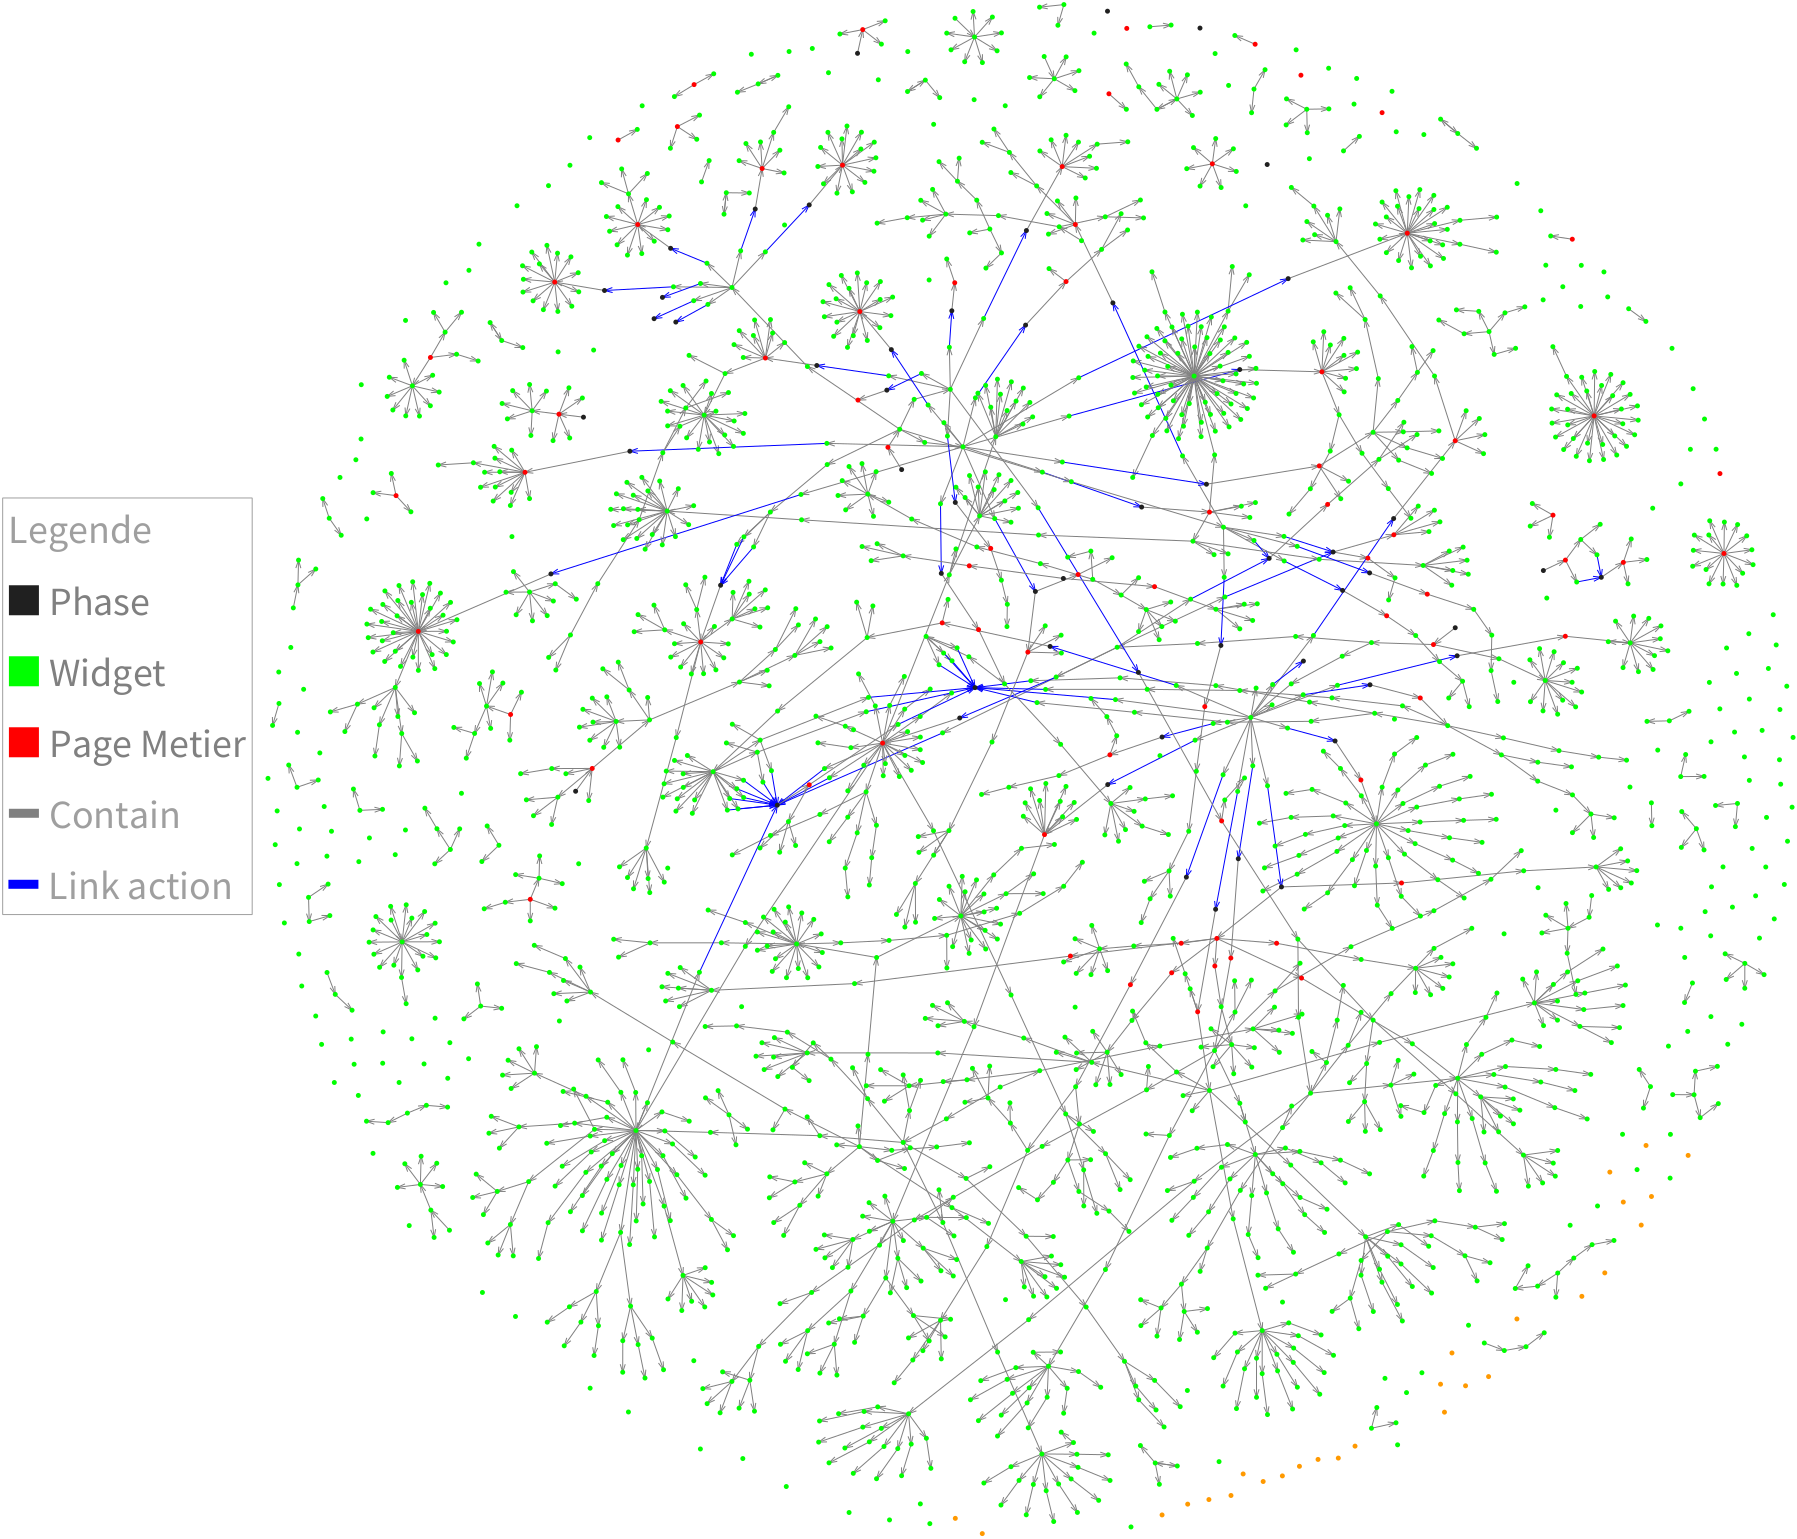
\includegraphics{figures/firework.png}
\caption{Représentation de l'application \emph{bac à sable} dans sa
globalité}\label{firework}
\end{figure}
}

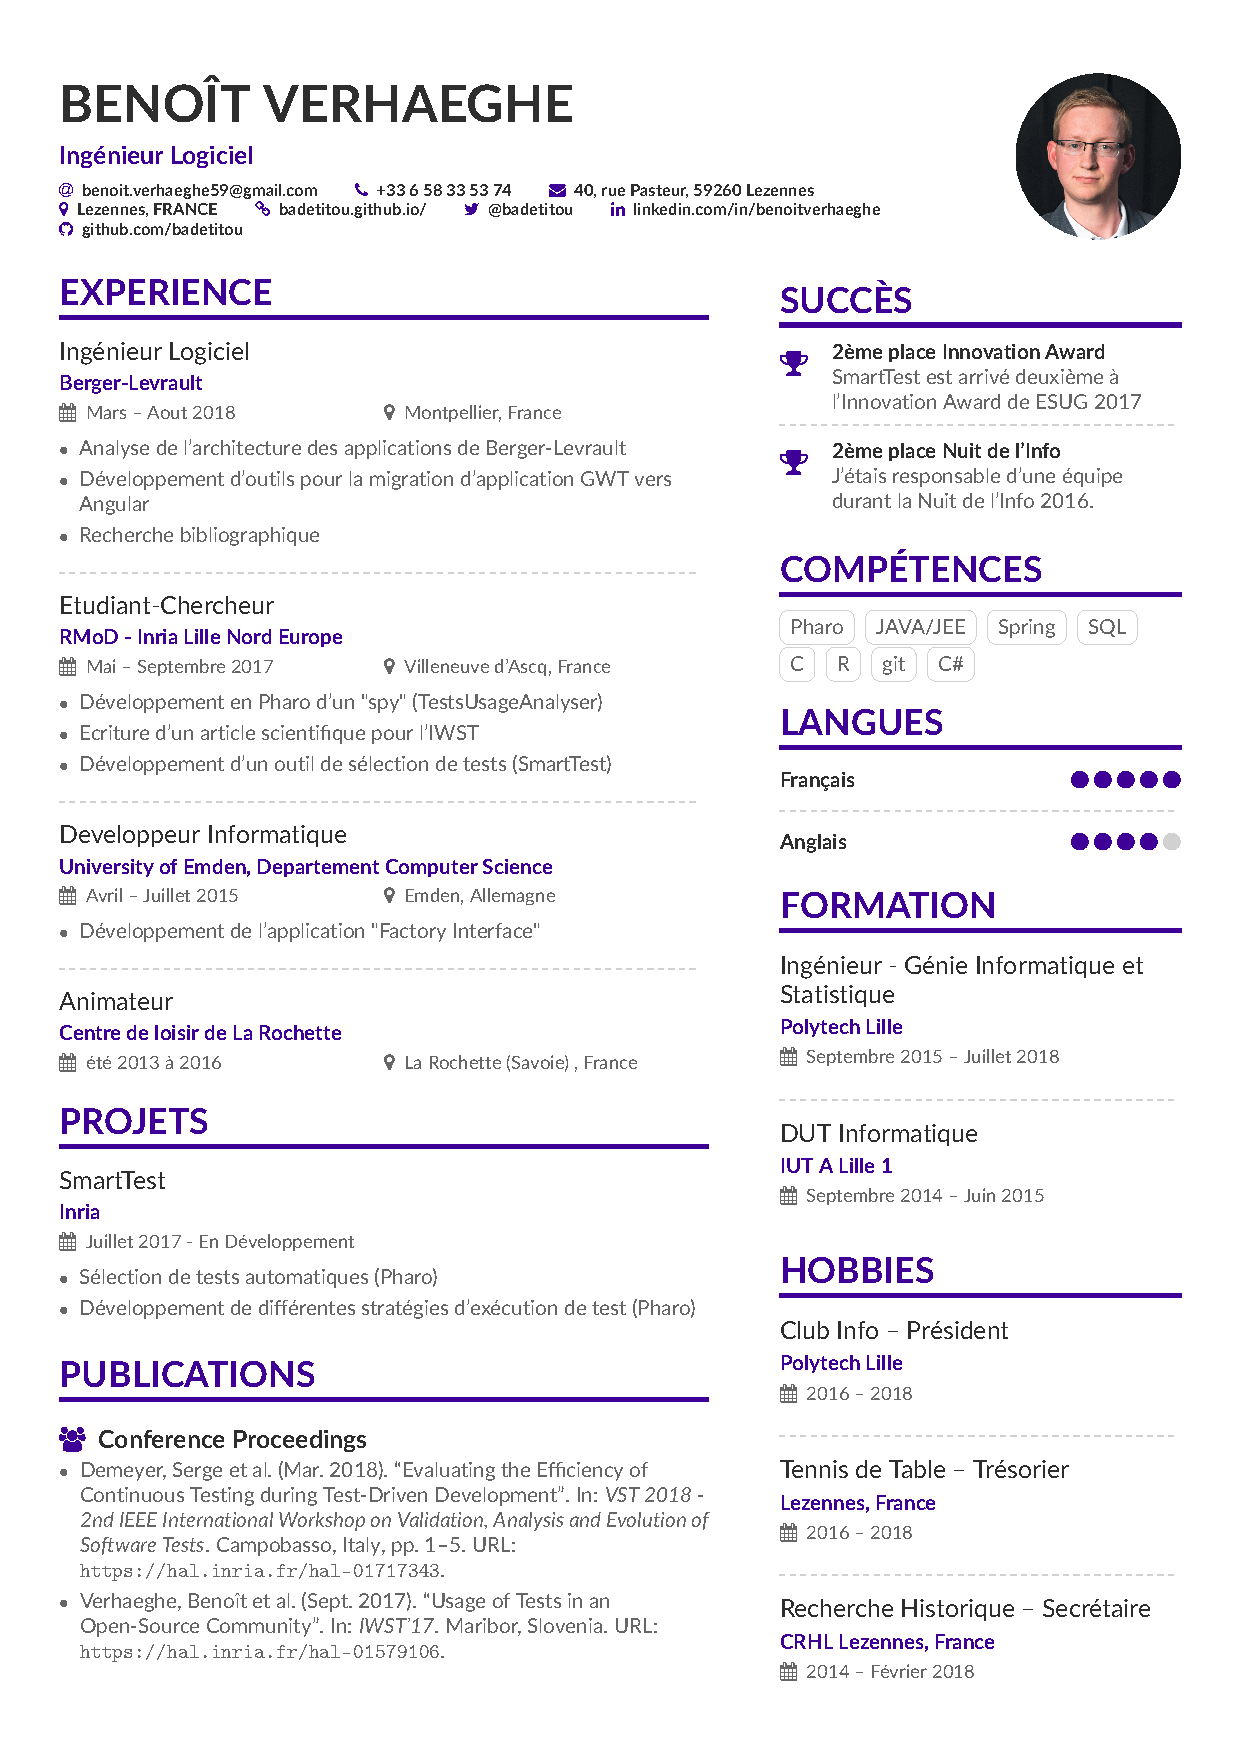
\includegraphics[width=0.9\textwidth,height=\textheight]{cv/cv.pdf} \#
Résumé

\hypertarget{franuxe7ais}{%
\subsection{Français}\label{franuxe7ais}}

Berger-Levrault est une entreprise majeure dans le monde de l'édition de
logiciel. Dans le cadre de l'évolution de ses applications, elle
souhaite changer le langage d'implémentation de ces derniers. Pour cela,
un travail préliminaire a été mené en Projet de Fin d'Études (PFE) où
l'on a étudié une application de démonstration (application \emph{``bac
à sable''}) qui reprend les principes d'organisation des applications de
Berger-Levrault. Le but de ce stage était de vérifier que les résultats
de l'étude préalable réalisée durant le PFE peut être appliqué grandeur
nature sur des applications en production de Berger-Levrault et définir
et implémenter une stratégie pour effectuer la migration des
applications. Lors de ce projet, nous avons notamment ;

\begin{itemize}
\tightlist
\item
  Modélisé des interfaces graphiques d'applications client de
  Berger-Levrault. Le but de cette modélisation est de fournir le
  maximum d'information sur les écrans de l'application pour permettre
  une réimplémentation (semi-)automatique dans un autre langage ;
\item
  Extrait automatiquement des composants des différents écrans de
  l'application;
\item
  Extrait une carte de navigation entre ces écrans (quel écran permet de
  passer à quel autre écran) ;
\item
  Définit une stratégie, passant par l'utilisation de modèles, pour
  effectuer la migration d'une application disposant d'une interface
  graphique
\item
  Réalisé un état de l'art sur le domaine de la migration d'application.
\item
  Migré l'application \emph{bac à sable} de GWT vers Angular.
\end{itemize}

\hypertarget{anglais}{%
\subsection{Anglais}\label{anglais}}
